\subsection{Views}

Document architecture using your selected views (at least logical, process and development) through diagrams and supporting/explaining text.	

\subsection{Logic view} 
The logic view provide an overview over the requirements over the principle of the game process. This figure show a decomposition of the logic of the game process and the relationship between these elements.

\begin{figure}[ht!]
	\centering
	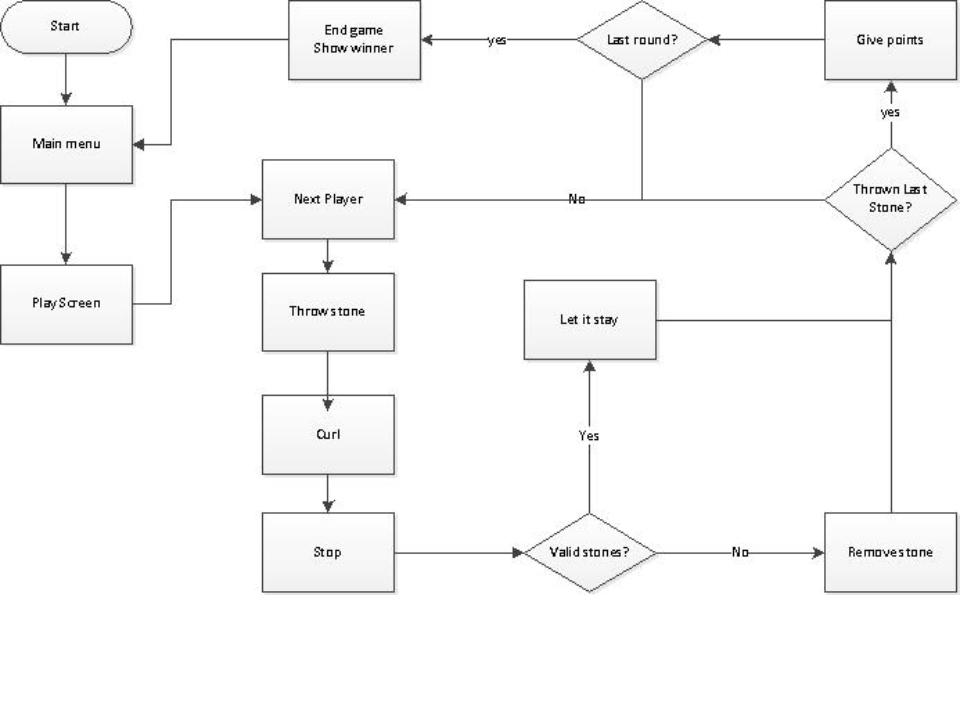
\includegraphics[width=150mm]{view.jpg}
	\caption{Logic view}
	\label{fig:view}
\end{figure}

\subsection{Process view}


\newpage
\begin{figure}[ht!]
	\centering
	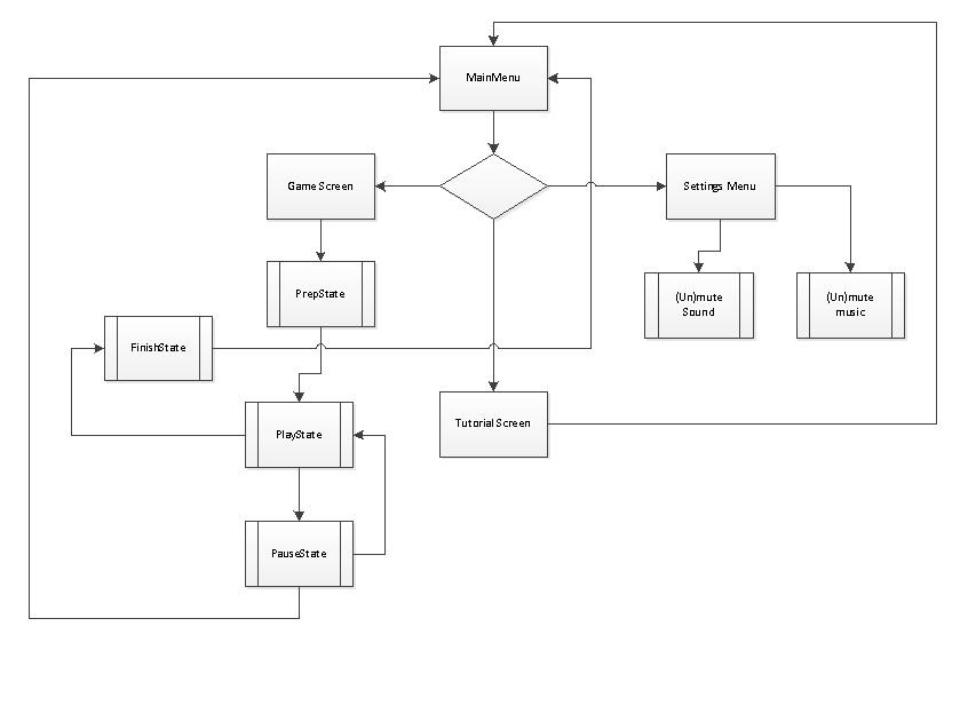
\includegraphics[width=150mm]{viewpoint.jpg}
	\caption{Process view}
	\label{fig:viewpoint}
\end{figure}

\subsection{Development view}
With the CurlingGame project at the base, it extends into three packages - model, viewactivities and the gamestate. Our model package takes care the model objects, as the curlingstone and the track, and is related to the Game class which draws and updates models. Our gamestate package holds all the viewcontrollers of the project. GameSettings is related to the game to change final variables such as how many balls to play with. Pause/Settings is an activity that pauses the game and brings up a settings-activity on top of the game activity. Finally, the Game class runs, draws, updates, and controls the entire game and other classes. Our project also utilizes the sheep API.

\newpage
\begin{figure}[ht!]
	\centering
	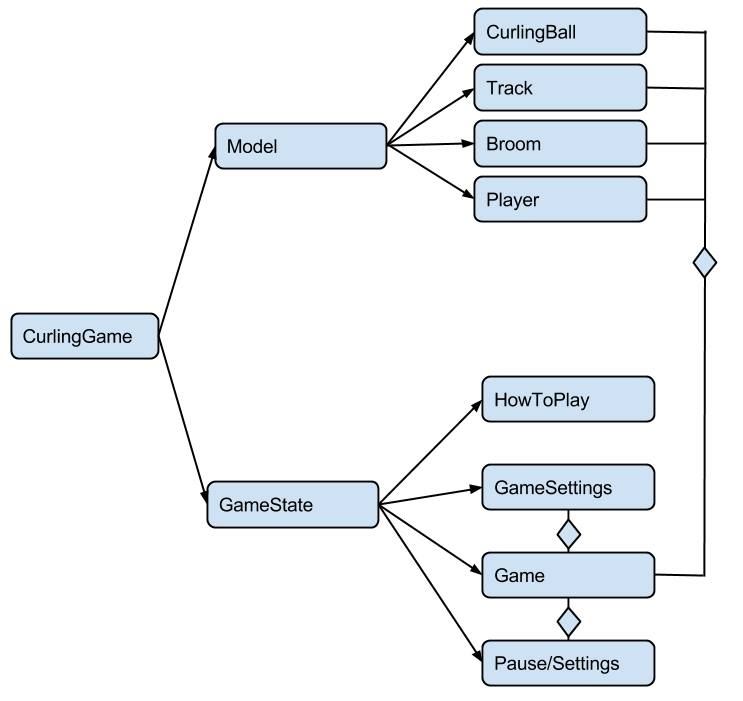
\includegraphics[width=150mm]{development_view.jpg}
	\caption{Development view}
	\label{fig:viewpoint}
\end{figure}